
\documentclass[oneside,a4paper]{book}
%\pagestyle{headings}


%=============================================================================

\usepackage{amsthm}
\usepackage{xspace}
\usepackage{float}
\usepackage{ifthen}
\usepackage{amsbsy}
\usepackage{amssymb}
\usepackage{balance}
\usepackage{booktabs}
\usepackage{graphicx}
\usepackage{rotating}
\usepackage{multirow}
\usepackage{needspace}
\usepackage{microtype}
\usepackage{bold-extra}
\usepackage{geometry}
\usepackage{varioref}
\usepackage{xcolor}
\usepackage{textcomp}
\usepackage{listings}
\usepackage[normalem]{ulem} %emphasize still italic
\usepackage{ucs}
\usepackage{booktabs}

% \usepackage[utf8]{inputenc}
% \usepackage[htt]{hyphenat}
\usepackage{times}
\usepackage{url}
\usepackage{alltt}
\usepackage{amsmath}
\usepackage{xfrac}
\usepackage{subfigure}
\usepackage{appendix}
\usepackage{stmaryrd}   % for the \shortuparrow
\usepackage[utopia]{quotchap}

\usepackage{setspace}
\usepackage[numbers, sort&compress]{natbib}
\usepackage{mdwlist}        % support for better spaced lists
% allows for temporary adjustment of side margins
\usepackage{chngpage}
\usepackage[normalem]{ulem} 

% constants

\newcounter{qcounter}

% commands
\newcommand{\n}{$\cdot$}
\newcommand{\y}{\checkmark}
\newcommand{\subscript}[1]{$_{\textrm{\footnotesize{#1}}}$}
\newcommand{\superscript}[1]{$^{\textrm{\footnotesize{#1}}}$}
\newcommand{\vertical}[1]{\raisebox{-4em}{\begin{sideways}{#1}\end{sideways}}}

\newboolean{showedits}
\setboolean{showedits}{true} % toggle to show or hide edits
\ifthenelse{\boolean{showedits}}
{
       \newcommand{\ugh}[1]{\textcolor{red}{\uwave{#1}}} % please rephrase
       \newcommand{\ins}[1]{\textcolor{blue}{\uline{#1}}} % please insert
       \newcommand{\del}[1]{\textcolor{red}{\sout{#1}}} % please delete
       \newcommand{\chg}[2]{\textcolor{red}{\sout{#1}}{\ra}\textcolor{blue}{\uline{#2}}} % please change
}{
       \newcommand{\ugh}[1]{#1} % please rephrase
       \newcommand{\ins}[1]{#1} % please insert
       \newcommand{\del}[1]{} % please delete
       \newcommand{\chg}[2]{#2}
}


% ============================================================================
% Put edit comments in a really ugly standout display

\usepackage{xcolor}
\usepackage[normalem]{ulem}
\newcommand{\ra}{$\rightarrow$}


% comments \nb{label}{color}{text}
\newboolean{showcomments}
\setboolean{showcomments}{true}
\ifthenelse{\boolean{showcomments}}
    {\newcommand{\nb}[3]{
        {\colorbox{#2}{\bfseries\sffamily\scriptsize\textcolor{white}{#1}}}
        {\textcolor{#2}{\sf\small$\blacktriangleright$\textit{#3}$\blacktriangleleft$}}}
     \newcommand{\version}{\emph{\scriptsize$-$Id$-$}}
%	 \newcommand{\ugh}[1]{\textcolor{red}{\uwave{#1}}} % please rephrase
%	 \newcommand{\ins}[1]{\textcolor{blue}{\uline{#1}}} % please insert
%	 \newcommand{\del}[1]{\textcolor{red}{\sout{#1}}} % please delete
%	 \newcommand{\chg}[2]{\textcolor{red}{\sout{#1}}{\ra}\textcolor{blue}{\uline{#2}}} % please change
	 \newcommand{\chk}[1]{\textcolor{ForestGreen}{#1}} % changed, please check
	}
    {\newcommand{\nb}[3]{}
     \newcommand{\version}{}
	\newcommand{\chk}[1]{} % changed, please check
	}

% ============================================================================
% Make quotes be italic
\renewenvironment{quote}
    {\list{}{\rightmargin\leftmargin}%
     \item\relax\begin{it}}
    {\end{it}\endlist}

\newcommand{\ttimes}{\ensuremath{\times}}

%=============================================================================

\newcommand{\needlines}[1]{\Needspace{#1\baselineskip}}

% source code
\usepackage{xcolor}
\usepackage{textcomp}
\usepackage{listings}
\definecolor{source}{gray}{0.9}
\lstset{
	language={},
	% characters
	tabsize=3,
	upquote=true,
	escapechar={!},
	keepspaces=true,
	breaklines=false,
	alsoletter={:},
	breakautoindent=true,
	columns=fullflexible,
	showstringspaces=false,
	basicstyle=\footnotesize\ttfamily,
	% background
	frame=single,
    framerule=0pt,
	backgroundcolor=\color{source},
	% numbering
	numbersep=5pt,
	numberstyle=\tiny,
	numberfirstline=true,
	% captioning
	captionpos=b,
	numberbychapter=false,
	% formatting (html)
	moredelim=[is][\textbf]{<b>}{</b>},
	moredelim=[is][\textit]{<i>}{</i>},
	moredelim=[is][\uline]{<u>}{</u>}}
\newcommand{\ct}{\lstinline[backgroundcolor=\color{white},basicstyle=\footnotesize\ttfamily]}
\newcommand{\lct}[1]{{\small\tt #1}}


%----------------------------------------------------------------------------
% references
\newcommand{\tabref}[1]{\hyperref[{tab:#1}]{Table~\ref*{tab:#1}}}
\newcommand{\figref}[1]{\hyperref[{fig:#1}]{Figure~\ref*{fig:#1}}}
\newcommand{\secref}[1]{\hyperref[{sec:#1}]{Section~\ref*{sec:#1}}}
\newcommand{\lstref}[1]{\hyperref[{lst:#1}]{Listing~\ref*{lst:#1}}}
\newcommand{\charef}[1]{\hyperref[{cha:#1}]{Chapter~\ref*{cha:#1}}}
%----------------------------------------------------------------------------

% abbreviations
\tracingcolors 4
\setcounter{tocdepth}{3}
\setcounter{secnumdepth}{3}
\newcommand{\ie}{\emph{i.e.,}\xspace}
\newcommand{\eg}{\emph{e.g.,}\xspace}
\newcommand{\etc}{\emph{etc.}\xspace}
\newcommand{\etal}{\emph{et al.}\xspace}


\newcommand{\newevenside}{
	\ifthenelse{\isodd{\thepage}}{\newpage}{
	\newpage
        \phantom{placeholder} % doesn't appear on page
	\thispagestyle{empty} % if want no header/footer
	\newpage
	}
}

\def\stretchfactor{1}
\newcommand{\mychapter}[1]{\setstretch{1}
    \chapter{#1}\setstretch{\stretchfactor}}

%----------------------------------------------------------------------------
\newcommand{\lessSpace}{\vspace{-1em}}
\DeclareGraphicsExtensions{.pdf,.png}
\graphicspath{{images/}}
\newcommand{\fig}[4]{
	\begin{figure}[#1]
		\centering
		\includegraphics[width=#2\textwidth]{#3}
		\lessSpace
		\caption{\label{fig:#3}#4}
	\end{figure}}

% ===========================================================================


\newcommand{\thesistitle}{Automating high-quality translations for Mobile Apps}
\newcommand{\thesisauthor}{Wanzenried \& Stefan}
\newcommand{\thesisleiter}{Prof. Dr. Philippe Cudr\'{e}-Mauroux}
\newcommand{\thesisasst}{Roman Prokofyev}
\newcommand{\thesissubtitle}{}
\newcommand{\thesisdate}{May 2016}



% ===========================================================================

\usepackage[ colorlinks=true, urlcolor=black, linkcolor=black,
			citecolor=black, bookmarksnumbered=true, bookmarks=true,
			plainpages=false,
			pdftitle={\thesistitle}, pdfauthor={\thesisauthor},
			pdfsubject={\thesissubtitle}, pdfpagelabels]{hyperref}

\newcommand{\hrref}[2]{\hyperref}
% ===========================================================================
% ===========================================================================


% D O C U M E N T
% % % % % % % % % % % % % % % % % % % % % % % % % % % % % % % % % %
\begin{document}

% T I T L E
% % % % % % % % % % % % % % % % % % % % % % % % % % % % % % % % % %
\begin{titlepage}  
  \begin{center}  
  
  \begin{figure}[t]  
  \vspace*{-2cm}        % to move header logo at the top 
  \center{
\includegraphics[scale=0.2]{logos/MSc_quer.png}}
  \vspace{0.4in}     
  \end{figure}

    \thispagestyle{empty}
    
    {\bfseries\Huge \thesistitle \par
    \Large \vspace{0.1in} \thesissubtitle \par}

    \vspace{0.3in} 
    \LARGE{\textbf{Master Thesis} \\}
    \vspace{0.4in}

    {\Large \thesisauthor \par from \par Bern BE, Switzerland}
    
    \vspace{0.3in}
%    {\Large Home University \par}
    {\Large Philosophisch-naturwissenschaftliche Fakult\"{a}t \\
            der Universit\"{a}t Bern \par}
    \vfill
    {\Large \thesisdate \par}
    \vspace{0.3in}
    %Leiter der Arbeit: \par
%   {\Large \thesisleiter, Research Group, Institute, University, Supervisor}\par
   {\Large \thesisleiter, eXascale Infolab, University of Fribourg, Switzerland, Supervisor}\par
   {\Large \thesisasst, eXascale Infolab, University of Fribourg, Switzerland, Assistant}
  

  \vspace{0.9in}
 
  % === Logos ==============================================     
  \begin{figure}[htp]
    \centering
    
\includegraphics[scale=0.30]{logos/UNI_Bern.png}\hfill
    
\includegraphics[scale=0.30]{logos/UNI_Neuenburg.png}\hfill
    
\includegraphics[scale=0.80]{logos/UNI_Fribourg.png}
  \end{figure}
  % === // Logos ===========================================    


  \end{center}

\end{titlepage}


% A B S T R A C T
% % % % % % % % % % % % % % % % % % % % % % % % % % % % % % % % % %
\chapter*{\centering Abstract}
\begin{quotation}
\noindent 
Every day, hundreds of mobile applications are added to stores such as Google Play or AppStore. Many of them are intended to be used internationally, and thus require translation of the interface. At the same time, many more mobile apps already available for download in these stores. Leveraging the translation bases of existing applications, we could immediately provide high-quality translations for new apps without need to go though a human-translation process. 

This project aims to extract and parse translations of existing applications to see if they can be used to translate new ones. A prototype application allows to translate existing apps from a given source to a target language. Translations are generated with different algorithms in statistical machine translation.
\end{quotation}
\clearpage


% C O N T E N T S 
% % % % % % % % % % % % % % % % % % % % % % % % % % % % % % % % % % % % % % % %
\tableofcontents

%%%%%%%%%%%%%%%%%%%%%%%%%%%%%%%%%%
%%%% NEW CHAPTER %%%%%%%%%%%%%%%%%%%%%
%%%%%%%%%%%%%%%%%%%%%%%%%%%%%%%%%%
\chapter{Introduction}
\label{cha:introduction}

Android, iPhone and Windows smart phones are available in countries all over the world. If an app is intended to be used internationally, translating it into multiple languages can be important to attract users. Users may only use the app if its text is available in their native language. Offering multiple languages is therefore crucial for paid apps to increase sales. However, translating an app requires additional effort. From a developers perspective, all strings must be isolated in order to replace them with different values for each supported language. Furthermore, translating text itself is a difficult task which usually requires the work of a professional translator.

The main idea of this thesis is to collect a lot of existing apps and extract their translations. Are we able to provide high quality translations with the help of Statistical Machine Translation (SMT)? To reduce the scope of different mobile operating systems and languages, we focus on automatic translations of Android apps from English to French and German. From now on, the term \emph{app} in this thesis refers to a Android application. We have chosen French and German as target languages for the translations because they are natively spoken in Switzerland, which makes understanding the produced results easier. %Also our data analysis showed that these two languages are very popular.% 
SMT is the dominant approach in automating translations and used by services like ``Google Translate''\footnote{\url{https://translate.google.com}} and Microsoft's ``Bing Translator''\footnote{\url{https://www.bing.com/translator}}. In this thesis, we use different SMT algorithms to produce translations and compare their results, both manually and automatically. A prototype web application is built which serves as a playground to translate strings and apps.

\chapter{Problem Analysis}
\label{cha:problem_analysis}

This chapter answers the question why it is important to offer multiple languages for apps.  

%Furthermore we take a look at existing translation services and briefly introduce how the service developed with this thesis is going to work. %

\section{Importance of Translating Mobile Apps}

%https://web.archive.org/web/20150402231142/http://www.distimo.com/blog/2012_10_publication-the-impact-of-app-translations/%

%https://web.archive.org/web/20150327084808/http://www.distimo.com/publications%

Google encourages developers to localize their apps on their localization checklist.\footnote{Android localization checklist: \url{http://developer.android.com/distribute/tools/localization-checklist.html}}

\begin{quote}
Android and Google Play offer you a worldwide audience for your apps, with an addressable user base that's growing very rapidly in countries such as Japan, Korea, India, Brazil, and Russia. We strongly encourage you to localize as it can maximize your apps’ distribution potential resulting in ratings from users around the world.
\end{quote}

The developer should first identify the countries where the app will be distributed based on the overall market size and opportunity, app category, local pricing etc. According to the identified countries, the supported languages are determined. Ideally an app supports multiple languages already before the first version is available in the app store. Users may install the app only once and forget about it, if they are not able to understand it.

Since 2013, Google offers an (human-based) app translation service to developers.\footnote{Android Developers Blog post about Googles translation service: \url{http://android-developers.blogspot.ch/2013/11/app-translation-service-now-available.html}} Several developers who participated at the pilot program shared their results after translating their apps:

\begin{itemize}
\item The developers of Zombie Ragdoll\footnote{Game Zombie Ragdoll in the Google Playstore: \url{https://play.google.com/store/apps/details?id=com.rvappstudios.zombieragdoll}} used this tool to launch their new game simultaneously in 20 languages in August 2013. When they combined app translation with local marketing campaigns, they found that 80\% of their installs came from non-English-language users.
\item Dating app SayHi\footnote{Dating app SayHi! in the Google Playstore: \url{https://play.google.com/store/apps/details?id=com.unearby.sayhi}} Chat expanded into 13 additional languages using the App Translation Service. They saw 120\% install growth in localized markets and improved user reviews of the professionally translated UI.
\item The developer of card game G4A Indian Rummy\footnote{Card game Indian Rummy \url{https://play.google.com/store/apps/details?id=org.games4all.android.games.indianrummy.prod}} found that the App Translation Service was easier to use than their previous translation methods, and saw a 300\% increase with user engagement in localized apps.
\end{itemize}


In 2012, ``App Annie'' \footnote{\url{https://www.appannie.com}} (former called ``Distimo''), published a study where they analysed the impact of translations to iPhone apps.\footnote{App Annie's study The impact of app translations: \url{https://web.archive.org/web/20150327084808/http://www.distimo.com/publications}} They found out that the use of native language is still limited in several countries, for example Italy, Russia or Brazil. Native-only apps are mostly used in Asian countries (see Figure \ref{fig:problem_analysis_impact_languages}).
The study followed 200 iPhone apps that introduced native language support in a market and observed their growth. Only one week after the local language support was introduced with an app update, downloading increased by 128\% and revenue by 26\%.

%Another case-study by David Janner from make app magazine\footnote{\url{http://makeappmag.com/iphone-app-localization-keywords}} observed the impact of translating one single app.
%

\begin{figure}[H]
    \centering
    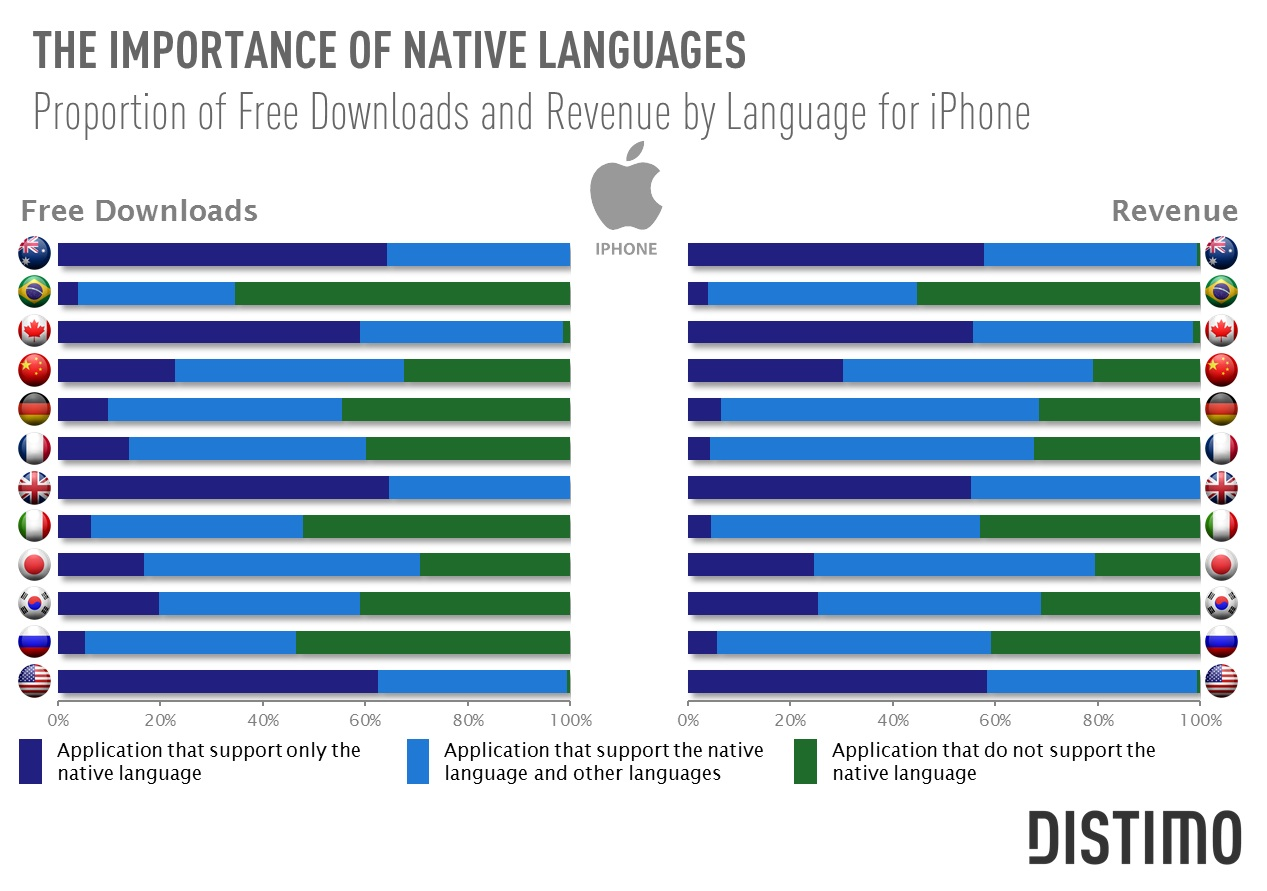
\includegraphics[width=0.8\textwidth]{images/problem_analysis_app_annie.jpg}
    \caption{Screenshot from the study ``The impact of app translations'' by App Annie showing the distribution of apps supporting native and other languages for the 12 top languages.}
    \label{fig:problem_analysis_impact_languages}
\end{figure}


\section{Translation Services}


\section{Statistical Machine Translation}

Machine translation has a long history, but over the last decade or two, its evolution has taken on a new direction - a direction that is mirrored in other subfields of natural language processing. This new direction is grounded in the premise that language is so rich and complex that it could never be fully analyzed and distilled into a set of rules, which are then encoded into a computer program. Instead, the new direction is to develop a machine that discovers the rules of translation automatically from a large corpus of translated text, by pairing the input and output of the translation process, and learning from the statistics over the data.\cite{smt_book_koehn}

%Statistical Machine Translation (SMT) is based on a large corpus of bilingual data. A translation model is trained to output the best possible translation according to some probabilistic function. In the context of this thesis it means that we learn a translation system from extracted translation of various apps.%

SMT translation models are usually trained on a large parallel corpus which is freely available on the web \footnote{\url{http://www.statmt.org/europarl/}}. The BLEU metric is then used to measure the quality of the produced translations. \cite{bleu_score}
There exists a recurring translation task of the ``Workshop on statistical machine translation'', which focuses on translating european language pairs by improving existing systems\footnote{\url{http://www.statmt.org/wmt15/translation-task.html}}.

In this thesis, we compare two different SMT algorithm and evaluate how they perform in the context of translating short sentences of mobile apps. The models are therefore applied on a much smaller data set than usual.

\section{Challenges}


\begin{itemize}
\item Quality of existing translations
\item Where and how to obtain large amount of apps
\item Hardware to train the translation models
\item How many data is needed to produce good results?
\item How can we measure good translations?
\end{itemize}



%\section{Android apps and internationalization}

%Android uses a key-value based approach to store translations and other resources in XML files\footnote{\url{http://developer.android.com/guide/topics/resources/localization.html}}. For each supported language, one XML file exists, containing the translated values to given keys. In the source code, a string is no longer hardcoded but referenced by a translation key.%

%\section{Challenges}%



\chapter{Related Work}
%In which we learn what have other done to address similar problems. For example, the work of Star \cite{Star89}

%Overview of SMT
%Has been done but not specific domain of short sentences mobile

This chapter provides an overview of Statistical Machine Translation (SMT). We consider two different models. The first one is called ``Statistical Phrase-Based Translation'' and was introduced in 2003 by Philipp Koehn et al. \cite{smt_phrase_based}\cite{smt_book_koehn} The second, more recent model, uses Deep Learning Neural Networks to perform translations. \cite{smt_deep_learning1} \cite{smt_deep_learning}

\section{Phrase-Based Machine Translation}
\label{sec:phrase_based_mt}
\subsection{Model}

Given the task to translate a sentence from a foreign language \(f = f_1, f_2, f_3..., f_m\) into an english sentence \(e = e_1, e_2, e_3 ..., e_n\), the translation model is based on the following probabilistic equation:

\[P(e|f)\]

To find the best english translation, the following equation is used (Bayes rule).

\[e_{best} = argmax_eP(e|f)\]
\[= argmax_e\frac{P(f|e)P(e)}{P(f)}\]
\[= argmax_e P(e|f)P(e)\]

where \(P(e)\) is called the \emph{language model}\footnote{\url{https://en.wikipedia.org/wiki/Language_model}} and \(P(f|e)\) is the \emph{translation model}.

The translation model is further decomposed:

\[p(\bar{f}_1^I|\bar{e}_1^I) = \prod_{i=1}^I \phi(\bar{f}_i^I|\bar{e}_i^I) d(start_i - end_{i-1} -1)\]

where \(\phi\) is called the \emph{phrase translation probability} and \(d\) is the \emph{reordering probability}.

The foreign sentence \emph{f} is broken up into \emph{I} phrases \(\bar{f}_i\). Each foreign phrase is translated into an English phrase \(\bar{e}_i\).

Reordering is handled by a \emph{distance based reordering model}. We define \(start_i\) as the position of the first word of the foreign input phrase that translates to the \emph{i}th English phrase, and \(end_i\) as the position of the last word of that foreign phrase. The reordering distance is the number of words skipped when taking foreign words out of sequence (see figure \ref{fig:related_work_phrase_based_reordering}).

\begin{figure}[H]
    \centering
    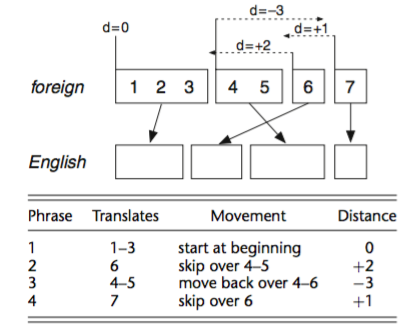
\includegraphics[width=0.4\textwidth]{images/related_work_phrase_based_reordering.png}
    \caption{Distance based reordering \cite{smt_book_koehn}}
    \label{fig:related_work_phrase_based_reordering}
\end{figure}

\emph{d} is turned into a proper probability distribution by applying an exponentially decaying cost function \(d(x) = \alpha^{|x|}\) with \(\alpha \epsilon [0,1]\). This means that movements of phrases over large distances are more expensive than shorter movements or no movement at all.


\subsection{Learning a Phrase Translation Table}

Building a phrase translation table involves three stages:
\begin{enumerate}
\item \textbf{Word alignment} The words of each sentence from the parallel corpus of the foreign and English language must be aligned in order to extract phrase pairs. The alignment is typically done by using one of the IBM models.\footnote{IBM word alignment models: \url{https://en.wikipedia.org/wiki/IBM_alignment_models}} Figure \ref{fig:related_work_word_alignment} shows an example of word alignment for a top term from our corpus.
\item \textbf{Extraciton of phrase pairs} Extract all phrase pairs of parallel sentences that are consistent with word alignment. A phrase pair (\(\bar{f}\),\(\bar{e}\)) is consistent with an alignment \emph{A}, if all words \(f_1,...,f_n\) in \(\bar{f}\) that have alignment points in \emph{A} have these with words \(e_1,...,e_n\) in \(\bar{e}\) and vice versa.
\item \textbf{Scoring phrase pairs} Assign probabilities to phrase translations.
\end{enumerate}

\begin{figure}[H]
    \centering
    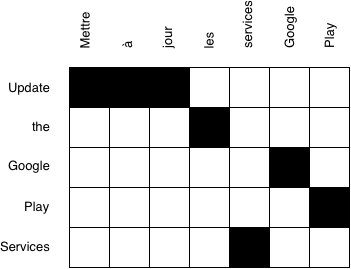
\includegraphics[width=0.4\textwidth]{images/related_work_word_alignment.png}
    \caption{Word alignment between a top term of our parallel Enlgish/French corpus.}
    \label{fig:related_work_word_alignment}
\end{figure}

\begin{figure}[H]
    \centering
    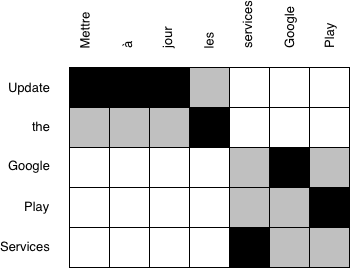
\includegraphics[width=0.4 \textwidth]{images/related_work_phrase_alignment.png}
    \caption{Extract phrase pairs consistent with word alignment.}
    \label{fig:related_work_phrase_alignment}
\end{figure}


We are able to extract the following phrase pairs from the example sentence:
\begin{itemize}
\item Update the Google Play Services / Mettre \a`a jour les services Google Play
\item Update / Mettre \a`a jour
\item Update the / Mettre \a`a jour les
\item Google Play Services / services Google Play
\item The Google Play Services / les services Google Play
\item Google Play / Google Play
\item Google / Google
\item Play / Play
\item Services / services
\item the / les
\end{itemize}
The last step is to estimate the phrase translation probabilities by the relative frequency:

\[\phi(\bar{f}|\bar{e}) = \frac{count(\bar{e},\bar{f})}{\sum_{\bar{f}_i }count(\bar{e},\bar{f}_i)}\]
These probabilities are put in the phrase translation table, together with the English and foreign phrase (see Figure \ref{fig:phrase_table_example}).

\begin{table}[H]
\centering
\begin{tabular}{@{}lr@{}}
\toprule
Foreign Phrase & \(\phi(\bar{f}|\bar{e})\)  \\ \midrule
param\a`etres     & 0.9         \\
r\a'eglages       & 0.36        \\
configuration  & 0.15        \\ \bottomrule
\end{tabular}
\caption{Example of a phrase translation table containing the estimated probabilities for translating the English word ``Setting'' to French.}
\label{fig:phrase_table_example}
\end{table}


\subsection{Decoding}
\label{sec:phrase_based_decoding}

Decoding is the process of finding a translation for a given input sentence. 
%Due to the big size of a phrase translation table, the search method is heuristic based. This means that the search algorithm can't explore the entire search space and therefore there is no guarantee that it will return the best translation.%
Recall the model to compute the translation probability:

\[e_{best} = argmax_{e} \prod_{i=1}^I \phi(\bar{f}_i|\bar{e}_i) d(start_i - end_{i-1} -1) p_{LM}(e)\]

\begin{itemize}
\item \textbf{Phrase translation} Pick phrase \(\bar{f}_i\) to be translated as phrase \(\bar{e}_i\) by looking up the score from the phrase translation table.
\item \textbf{Reordering} The previous phrase ended in \(end_{i-1}\), the current phrase starts at \(start_i\). Compute \(d(start_i - end_{i-1} -1)\)
\item \textbf{Language model} For a \emph{n}-gram model, we need to keep track of the last \(n - 1\) words. The score is computed for every added word \(w_i\): \(p_{LM}(w_i|w_i - (n-1), ..., w_{i-1})\)
\end{itemize}
The algorithm reads the input sentence from left to right and creates a new hypothesis by picking any phrase translation at a time. The score is computed incrementally for each partial hypothesis. This is repeated recursively until all hypotheses have been expanded. A hypothesis covering all input words cannot be expanded further and forms and end point in the search graph (Figure \ref{fig:related_work_hypothesis}). To get the best translation, we pick the completed hypothesis with the highest probability score and backtrack through the search graph. 

\begin{figure}[H]
    \centering
    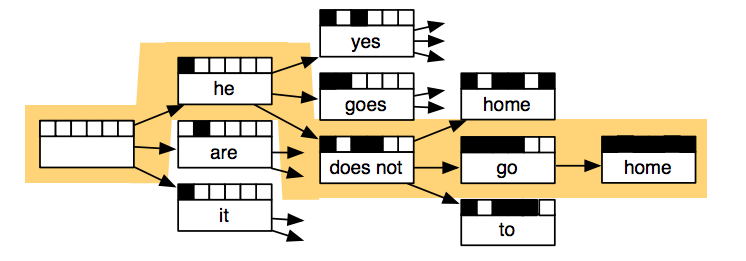
\includegraphics[width=0.7\textwidth]{images/related_work_hypothesis.png}
    \caption{Example: Created hypothesis by translating the German sentence ``er geht ja nicht nach hause'' to English. The squares on top indicate a coverage vector of translated German words (filled black if covered). \cite{smt_book_koehn}}
    \label{fig:related_work_hypothesis}
\end{figure}
This process creates an exponential number of hypothesis. To reduce the search space, the following methods are applied:

\begin{itemize}
\item \textbf{Recombination} Two hypothesis paths lead to two matching hypotheses, e.g. have the same English words in the output. The worse hypothesis is dropped.
\item \textbf{Stack Pruning} Bad hypotheses are removed early. Hypothesis that have translated the same number of input words are put into a stack, so that they are comparable. The number of hypotheses in a stack is limited, for example by keeping only \emph{k} hypotheses according to a score. This score is a combination of the partial probability score and a future cost estimation of the remaining sentence.
\end{itemize}


\section{Deep Learning Neural Networks}

Translating with neural networks is based on a encoder-decoder architecture. \cite{smt_deep_learning1} \cite{smt_deep_learning} Two recurrent neural networks (RNN)\footnote{\url{https://en.wikipedia.org/wiki/Recurrent_neural_network}} are involved: The first RNN encodes a variable-length sequence into a fixed-length vector representation. The second RNN decodes a given fixed-length vector back into a variable-length sequence.
We first describe shortly the working of a RNN before explaining the encoder-decoder architecture in more detail. Beside the papers, we also want to mention a blog post\footnote{\url{https://devblogs.nvidia.com/parallelforall/introduction-neural-machine-translation-with-gpus/}} by NVIDIA which offers a very detailed explanation of the model.


\subsection{Recurrent Neural Network}

A recurrent neural network is a class of artificial neural network where connections between units form a directed cycle. It consists of a hidden state \(h\) and an optional output \(y\) which operates on a variable-length sequence \( x = (x_1, ..., x_n)\). At each time step \(t\), the hidden state \(h_{t}\) is updated by:

\[  h_{t} = f(h_{t-1}, x_t) \]
where \(f\) is a non-linear activation function. The function described in the paper by Cho et al. \cite{smt_deep_learning1} is motivated by a long short-term memory (LSTM) unit\footnote{\url{https://en.wikipedia.org/wiki/Long_short-term_memory}}, but much simpler to compute and implement.

An RNN can learn a probability distribution over a sequence by being trained to predict the next symbol in a sequence. In this case, the output at each timestep \(t\) is the conditional distribution \( p(x_t | x_{t-1}, ... , x_1) \).


\subsection{Encoder}

The encoder RNN reads each word of the source sentence sequentially in the form of a ``One-hot vector''. This binary vector has the size of the vocabulary and zeros everywhere except a \(1\) at the position corresponding to the index of the word in the source vocabulary.

The internal state \(h_t\) changes each time a new word is read:

\[  h_{t} = f(h_{t-1}, x_t) \]
At the end of processing each word, the hidden state or the RNN is a summary \(c\) of the source sentence (see Figure \ref{fig:related_work_encoder}). 

\begin{figure}[H]
    \centering
    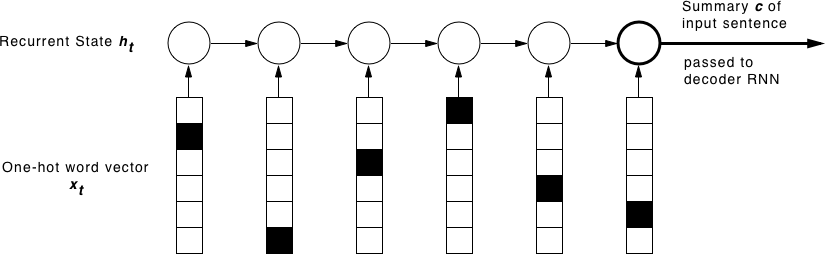
\includegraphics[width=0.85\textwidth]{images/related_work_encoder.png}
    \caption{Overview of the encoder RNN: The hidden state \(h_t\) (circle) is computed by taking the previous hidden state and a new word vector \(x_t\). At the end of the sentence, the hidden state is a summary \(c\) of the input sentence, that is passed to the decoder RNN.}
    \label{fig:related_work_encoder}
\end{figure}
It is very interesting how the summary vector \(c\) looks like. Sutskever et al. \cite{smt_deep_learning} projected multiple summary vectors two a two-dimensional space (see Figure \ref{fig:related_work_summary_vector}). Their plot shows that similar sentences are close together in the summary vector space.

\begin{figure}[H]
    \centering
    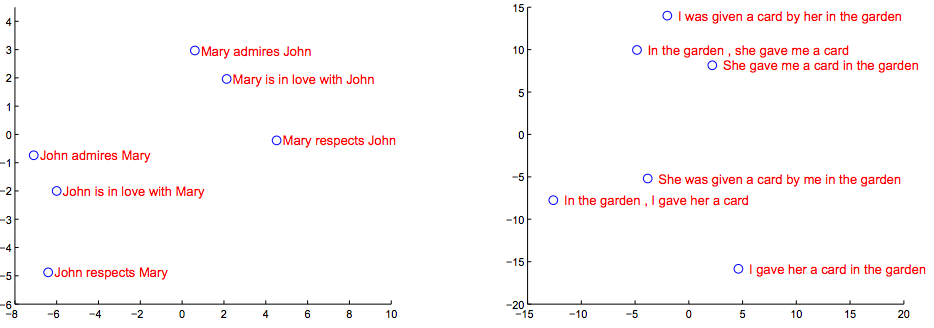
\includegraphics[width=0.95\textwidth]{images/related_work_pca_summary_vector.png}
    \caption{2D visualization of source sentences in the summary vectors space \cite{smt_deep_learning}. Similar sentences in terms of syntax and semantics are grouped together.}
    \label{fig:related_work_summary_vector}
\end{figure}


\subsection{Decoder}

The decoder is another RNN which is trained to generate the output sentence by predicting the next word \(y_t\) given the hidden state \(h_t\). Both \(y_t\) and \(h_t\) are conditioned on \(y_{t-1}\) and the summary vector \(c\) given from the encoder RNN. The hidden state of the decoder is computed by

\[  h_t = f(h_{t-1}, y_{t-1}, c) \]
The conditional distribution of the next target word is

\[ P(y_t|y_{t-1},y_{t-2},...,y_1,c) = g(h_t, y_{t-1}, c) \]
for given activation functions \(f\) and \(g\). The latter must produce valid probabilities.

\subsection{Training}

The proposed encoder-decoder system is trained by maximizing the log-likelihood\footnote{\url{https://en.wikipedia.org/wiki/Likelihood_function}} of the training corpus. Training requires a parallel corpus \(C\) of source and target sentences \((X^n, Y^n)\). The sentences are represented as sequence of one-hot vectors. We can compute the conditional log-probability of \(Y^n\) given \(X^n\) by \( log P(Y^n|X^n, \theta) \). The log-likelihood of the training corpus is written as:

\[ L(C,\theta) = \frac{1}{N} \sum_{n=1}^N log P(Y^n|X^n, \theta) \]
where \(N\) is the number of training samples and \(\theta\) is the set of model parameters.
Maximizing the log-likelihood function can be done by using stochastic gradient descent\footnote{\url{https://en.wikipedia.org/wiki/Stochastic_gradient_descent}}.

\chapter{Data Analysis}

\section{Apps}

A total of 698 free Android apps were collected from various categories\footnote{Click on Categories to see a list of available categories at:  \url{https://play.google.com/store/apps?hl=en}}, ensuring a good mix of different translations. Most of them were chosen randomly beside the top apps, mostly from Google. Figure \ref{fig:data_analysis_top_apps_en} shows the top ten apps according to the number of available english translations. Note that the counts indicate the number of effective translations after eliminating uninteresting data during pre-processing the corpus (see chapter \ref{cha:data_extraction_prep_storage}). Most of the apps have similar counts for all the three languages. Surprisingly, some apps provide more translations for german and french than english. Different counts can happen because of:

\begin{enumerate}
\item Not all strings were translated to all languages. Some english words remain the same in the target language and don't need to be translated, e.g. E-Mail.
\item The XML files containing the translations are out of sync, e.g. the developer forgot to add a french translation.
\item Some translations were abandoned during pre-processing.
\end{enumerate}

34 apps did not isolate their strings in XML files (we assume that they are hardcoded in the programming code). This leaves a effective number of 664 apps where we could extract translations. However, 241 apps among them were not multilingual and therefore not useful for building translation systems. Unfortunately, apps are not marked as multi-language in the app store, so we only know if there are translations available after downloading and extracting the data.

\begin{figure}[H]
    \centering
    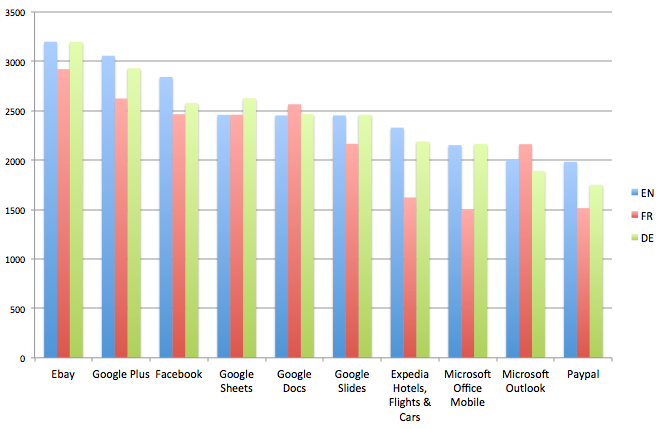
\includegraphics[width=0.75\textwidth]{images/data_analysis_top_apps_en.png}
    \caption{Top apps by the number of english translations}
    \label{fig:data_analysis_top_apps_en}
\end{figure}


\section{Languages}

We collected a total of 423 multilingual apps, offering its content at least for two languages. Figure \ref{fig:data_analysis_n_langs} shows the number of apps for the ten most used languages. French and German, where we focus on this thesis, are both in the top 4. The top apps are translated in many more languages. Overall, 117 different languages were available.

\begin{figure}[H]
    \centering
    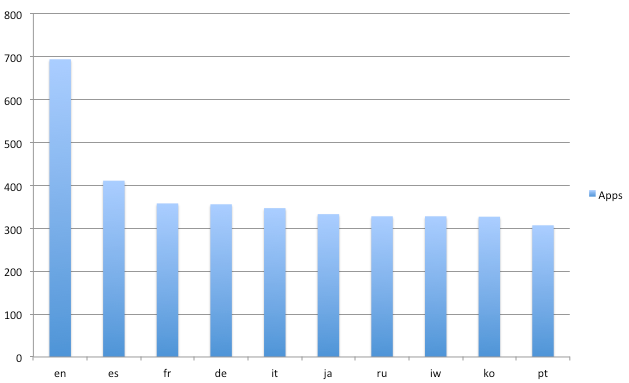
\includegraphics[width=0.75\textwidth]{images/data_analysis_languages_count.png}
    \caption{Number of apps available in the top ten languages.}
    \label{fig:data_analysis_n_langs}
\end{figure}


\section{Top Translations}


\begin{table}[H]
\centering
\resizebox{\textwidth}{!}{%
\begin{tabular}{@{}llllllll@{}}
\toprule
EN & Count &  & FR & Count &  & DE & Count \\ \midrule
Cancel & 1894 &  & Annuler & 1067 &  & Abbrechen & 886 \\
Done & 1230 &  & Supprimer & 745 &  & Google Play-Dienste aktivieren & 730 \\
Settings & 1102 &  & Connexion & 745 &  & Google Play-Dienste installieren & 728 \\
Search & 884 &  & Mettre à jour & 486 &  & Anmelden & 664 \\
Delete & 704 &  & Rechercher & 485 &  & Löschen & 664 \\
Enable Google Play services & 692 &  & Paramètres & 450 &  & Aktualisieren & 652 \\
Get Google Play services & 690 &  & Mettre à jour les services Google Play & 370 &  & Einstellungen & 569 \\
Log Out & 556 &  & Activer services google Play & 368 &  & Fertig & 548 \\
Update & 545 &  & Activer les services Google Play & 366 &  & Weiter & 484 \\
Share & 541 &  & Installer les services Google Play & 366 &  & Schliessen & 428 \\ \bottomrule
\end{tabular}
}
\caption{Top ten translations for english, french and german}
\label{table:data_analysis_top_terms}
\end{table}

\chapter{Data Extraction, Preparation and Storage}
\label{cha:data_extraction_prep_storage}

\section{Extract Translations}

An Android app has the form of a single binary file (suffix .apk). The XML files containing the translations are packed inside the .apk file. We used a software called ``Apktool''\footnote{\url{http://ibotpeaches.github.io/Apktool/}} to reverse engineer existing apps and extract the needed XML files.

\begin{figure}[H]
    \centering
    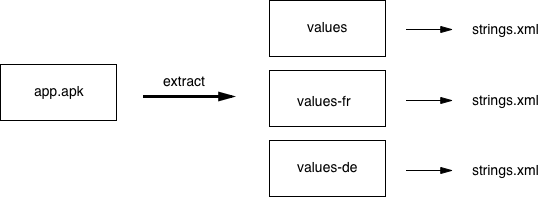
\includegraphics[width=0.6\textwidth]{images/data_extraction_xml.png}
    \caption{For each language, the translations are stored in a XML file}
    \label{fig:data_extraction_xml}
\end{figure}

Inside the \texttt{strings.xml} files, translations are stored key-value based. Each string has a unique key which holds the translation value for each language. Here is an example how an English XML file looks like:

\lstset{
language=XML,
morekeywords={encoding,resources,string }
}
\begin{lstlisting}
<?xml version="1.0" encoding="utf-8"?>
<resources>
    <string name="close_app">Close Application</string>
    <string name="back">Back</string>
    ...
</resources>
\end{lstlisting}


\section{Preprocess Translations}
\label{sec:preprocess_translations}
This task involves two parts. First of all, the translations are sanitized from unwanted information such as HTML tags. Some strings are omitted at this stage because they do not provide any meaningful value to the translation process, for example URLs or string placeholders. Secondly, the sanitized strings are tokenized so that they can be used by an SMT system.

\subsection{Sanitizing}

The following rules are used to get rid of unwanted translations or parts of it:

\begin{itemize}
\item Trim the string from newlines (\texttt{\textbackslash n}), tabs (\textbackslash t) or carriage return (\textbackslash r)
\item Strip any HTML tags
\item Omit strings that are URLs (starting with http or www)
\item Remove strings placeholders like \texttt{\%s} or \texttt{\%1\$s}
\item Ignore words with less than 3 characters
\item Finally, the resulting string is trimmed again from spaces and must contain at least one alphanumerical character
\end{itemize}


\subsection{Tokenization and Truecasing}

Tokenization is required to separate words from punctuation. Each token is separated by a space character: ``\texttt{Hi, my name is John.}'' becomes ``\texttt{Hi , my name is John .}''

After tokenizsation, truecasing was applied to our text corpus.\footnote{\url{https://en.wikipedia.org/wiki/Truecasing}} In contrast to lowercasing, truecasing determines the proper capitalization of words. This is done by first analyzing all data and then apply the most likely capitalization. It is especially useful for words starting a sentence, that are written uppercase in many languages. For example the word ``\texttt{This}'' starting a sentence will become ``\texttt{this}'', because it is usually written lowercase.


\section{Data storage}


\subsection{Parallel and Monolingual Corpus}

After pre-processing the translations, they are written to text files, one sentence per line. The corpus is split into parallel and monolingual data. A parallel corpus (often also called bitext) describes sentence aligned text-files of one language pair. All sentences must be aligned so that line x of the translation source language corresponds to line x of the target language. The sentences are shuffled before writing to get a random mix of translations of different apps. Most SMT system use this parallel data to train their translation model, so the parallel corpus can be reused multiple times.

In addition, data of any language is also stored monolingual. All sentences of one language are written into a single text file. This is for example used to build language models, which are an important part of a phrase-based translation model (see chapter \ref{sec:phrase_based_mt}).

\subsection{Apache Solr}
\label{sec:apache_solr}

We needed a simple way to store all translations, preferably with additional meta data, to perform data analysis and calculate statistics.
Apache Solr\footnote{\url{http://lucene.apache.org/solr/}} is used for this purpose. Solr is an open source text search platform built on top of Apache Lucene\footnote{\url{https://lucene.apache.org/core/}}. It allows to store the translations with additional meta data, such as the translation key and a unique app ID. Due to its way of indexing text data, Solr is very fast when querying for translation strings. Furthermore, built in tools allow to get nice statistics, for example the top terms grouped by language.

Solr is also used as Baseline translation system, where we translate strings with a simple algorithm directly from the collected data in Solr. (see chapter xy).

\subsubsection{Setup and Schema}

Solr offers so called ``Cores'' where each core manages a separate index, schema and configuration\footnote{\url{https://cwiki.apache.org/confluence/display/solr/Solr+Cores+and+solr.xml}}. In our setup we created one core per language and one document per translation string. The schema is identical for each core (language) and consist of the following fields:

\begin{itemize}
\item \textbf{id} Unique ID used by Solr to identify a document.
\item \textbf{app\_id} Each app must have a unique app-ID.
\item \textbf{key} The translation key from the XML file.
\item \textbf{value} The translation value corresponding to the above key.
\item \textbf{value\_lc} Again the translation value, additionally indexed with a special start- and ending delimiter. This allows to search for exact values.
\end{itemize}

\begin{figure}[H]
    \centering
    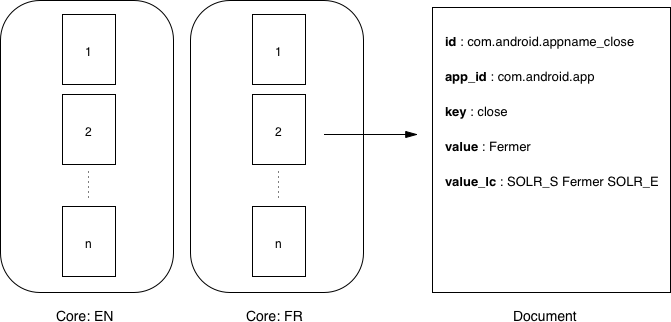
\includegraphics[width=0.8\textwidth]{images/data_extraction_solr_schema.png}
    \caption{Translations are stored in a document inside a separate core per language}
    \label{fig:data_extraction_solr_schema}
\end{figure}

The data in the \texttt{value} and \texttt{value\_lc} fields is stored tokenized and lowercased. The Solr Standard Tokenizer\footnote{\url{https://cwiki.apache.org/confluence/display/solr/Tokenizers\#Tokenizers-StandardTokenizer}} splits text into tokens, treating whitespace and punctuation as delimiters. Delimiter characters are discarded.

\subsubsection{Queries}

Solr offers a REST based interface to query the database. There is also a built in web application which allows to inspect results.
Here is an example query where we search for the string ``Log Out'' in the English core\footnote{You must be connected to the LAN of the University of Fribourg in order to access the referenced domain. Also note that the parameters should be fully url-encoded, this was omitted in this report for better readability.}. The maximum amount of results is set to 500 rows and the return type is JSON:
\\
\\
\url{http://diufpc114.unifr.ch:8983/solr/en/select?q=value:"Log\%20Out"&rows=500&wt=json&indent=true}
\\
\\
This query returns a total of 458 results. Note that there are not only exact matches returned, the term ``Log Out'' can occur as substring in a longer sentence (see figure xy). By default, Solr does not offer the possibility to return only exact matches. However, we can simulate this behaviour with the help of our \texttt{value\_lc} field, which indexed the string together with a special start- and end delimiter (\texttt{SOLR\_S} and \texttt{SOLR\_E}):
\\
\\
\url{http://diufpc114.unifr.ch:8983/solr/en/select?q=value_lc:"SOLR_S\%20Log Out\%20SOLR_E"&rows=500&wt=json&indent=true}
\\
\\
This query returns only 396 results. Note that the case of the search term doesn't matter and whitespace and punctuation are ignored. Executing the above query with the term ``log Out .'' returns the same results.

\begin{lstlisting}
"response": {
    "numFound": 458,
    "start": 0,
    "docs": [
      {
        "id": "com.flaregames.gargoyles_com_facebook_loginview_log_out_action",
        "app_id": "com.flaregames.gargoyles",
        "key": "com_facebook_loginview_log_out_action",
        "value": "Log Out",
        "value_lc": "SOLR_S Log Out SOLR_E"
      },
      {
        "id": "com.instagram.android_must_log_out_one_click_login",
        "app_id": "com.instagram.android",
        "key": "must_log_out_one_click_login",
        "value": "You must log out in order to login using this link.",
        "value_lc": "SOLR_S You must log out in order to login using this link. SOLR_E"
      },      ...
      ]
}
\end{lstlisting}


\chapter{Translation Process}

This chapter describes the different translation systems that were used to translate apps.

%The ``Baseline System'' makes direct use of the data stored in Solr and produces translations with a simple algorithm. The second system, ``Moses''\footnote{Moses SMT system: \url{http://www.statmt.org/moses/}}, is a open source phrase-based SMT software. Lastly ``Tensorflow''\footnote{Tensorflow: \url{https://www.tensorflow.org/}} was used to produce translations with the help of deep learning neural networks. Tensorflow is a software library for machine intelligence, recently released as open source by Google.%

\section{Baseline System}

The ``Baseline System'' makes direct use of the data stored in Solr and produces translations with a simple algorithm. Remember how the data is organized in Solr (see section \ref{sec:apache_solr}): Each translation is stored in a document with a fixed schema and each document belongs to one core. To lookup a translation, the following procedure is used:

\begin{enumerate}
\item Search the string to translate in the source language
\item Parse the result documents and extract the \texttt{app\_id} and \texttt{key} fields
\item Lookup translations in the target language by querying the target core with the collected \texttt{app\_id}s and \texttt{key}s.
\item Count the number of unique translations found. The best translation is the value that was mostly used.
\end{enumerate}


\subsection{Algorithm}

Given a string \(S = [ \; s_1  \; s_2  \; ...  \; s_n \; ]\) with words \(s_i\) in the source language, we want to produce a string \(T = [ \; t_1 \; t_2  \; ... \; t_n \; ]\) in the target language. The algorithm recursively tries to translate the longest substrings of \(S\) by looking up translations for the substrings in Solr. This process is repeated until there are left only single words \(s_i\) to translate.

\begin{enumerate}
\item Check if we find any translation for \(S\) directly. If so, return the translation and exit.
\item Start translating the longest substrings of \(S\). To build the substrings, we move a ``window'' of size \(length(S) - i\) from left to right over \(S\), where \(i\) is the iteration level. Let \(length(S) = 7\); the following two  substrings of length 6 are possible at the first iteration (\(i = 1\)):

\begin{center}
\( V_1 = [ \; s_1 \; s_2 \; s_3 \; s_4 \; s_5 \; s_6 \; ] \; [ \; s_7 \; ]\)

\( V_2 = [ \; s_1 \; ] \; [ \; s_2 \; s_3 \; s_4 \; s_5 \; s_6 \; s_7 \; ]\)
\end{center}

Now, we search for translations for all substrings in both variations \(V_1\) and \(V_2\). If there are no translations available, the substring (window) size is reduced by one for the second iteration (\(i = 2\)):

\begin{center}

\(  V_1 = [ \; s_1 \; s_2 \; s_3 \; s_4 \; s_5 \; ] \; [ \; s_6 \; s_7 \; ]\)

\( V_2 = [ \; s_1 \; ] \; [ \; s_2 \; s_3 \; s_4 \; s_5 \; s_6 \; ] \; [ \; s_7 \; ]\)

\( V_3 = [ \; s_1 \; s_2 \; ] \; [ \; s_3 \; s_4 \; s_5 \; s_6 \; s_7 \; ]\)

\end{center}

This process of reducing the substring length is repeated until we can translate a substring of at least one variation \(V_j\).

\item Let's consider what happens if there are translations available. For each variation \(V_j\), we count the number of available translations for their substrings \(\bar{S}_i\). We continue with the variation \(\tilde{V}\) having the highest total count of translations among their substrings:

\[ \tilde{V} = argmax\sum_i count\_translations(\bar{S}_i) \]

If there is a translation available for each substring \(\bar{S}_i\) of \(\tilde{V}\), we can build the output string \(T\) directly by concatenating the substring translations: 

\begin{center}
\(T = \bar{T}_1 \; \bar{T}_2 \; \bar{T}_3 \; ... \; \bar{T}_n\)
\end{center}

Otherwise, we build the output string \(T\) incremental: If there is no translation found for substring \(\bar{S}_i\), we set \(S = \bar{S}_i\) and recursively call the algorithm again. If there are left single words to translate and no translation exists, we insert the source word into \(T\) by setting \(t_i = s_i\).

\end{enumerate}

This simple algorithm works well for translating short words or sentences where a direct translation exists in the target language. On the other hand, it suffers from the following problems if translating substrings is necessary:

\begin{itemize}
\item The sentences or words for the translated substrings are inserted at the same position in \(T\) where they occurred in the source string. This won't produce good results since words often need to be reordered depending on the target language, e.g. in German // TODO Example
\item Bad translations can have a direct impact on the result. For example, due to an error or uncompleted translation in the XML files, the English word ``the'' could be mapped to a sentence with 20 words.
\end{itemize} 


\subsection{Example}

Let us translate the source string ``Open the settings to change your username'' from English to French.

\begin{enumerate}
\item Check for a direct translation: No French translation available.
\item Start translating the substrings. The upper index indicates the number of translations found:

\begin{center}
\(V_1\) = [ Open the settings to change your ] \(^0\) [ username ] \(^{28}\)

\(V_2\) = [ Open ] \(^{63}\) [ the settings to change your username ] \(^0\)
\end{center}

Continue with Variation 2 since the count (63 + 0) is higher than the count from Variation 1 (0 + 28).

\item We set \(T\) = [ ouvrir ] and \(S\) = [ the settings to change your username ] and go recursive. Again, there does not exist a translation for \(S\) directly so the substrings are built:

\begin{center}
\(V_1\) = [ the settings to change your ] \(^0\) [ username ] \(^{28}\)

\(V_2\) = [ the ] \(^{1}\) [ settings to change your username ] \(^0\)
\end{center}

\item \(T\) = [ ouvrir ... nom d'utilisateur ] ; \(S\) = [ the settings to change your ]

\begin{center}
\(V_1\) = [ the settings to change ] \(^0\) [ your ] \(^{2}\)

\(V_2\) = [ the ] \(^{1}\) [ settings to change your ] \(^0\)
\end{center}

\item \(T\) = [ ouvrir ... votre nom d'utilisateur ] ; \(S\) = [ the settings to change ]

\begin{center}
\(V_1\) = [ the settings to ] \(^0\) [ change ] \(^{26}\)

\(V_2\) = [ the ] \(^{1}\) [ settings to change ] \(^0\)
\end{center}

\item \(T\) = [ ouvrir ... modifier votre nom d'utilisateur ] ; \(S\) = [ the settings to ]

\begin{center}
\(V_1\) = [ the settings ] \(^5\) [ to ] \(^{2}\)

\(V_2\) = [ the ] \(^{1}\) [ settings to ] \(^0\)
\end{center}

\item \(T\) = [ ouvrir les param\`{e}tres vers modifier votre nom d'utilisateur ] ; \(S\) = [ ] 

%\begin{center}
%\(V_1\) = [ the ] \(^1\) [ settings ] \(^{48}\)
%\end{center}


% \item \(T\) = [ ouvrir les param\`{e}tres vers modifier votre nom d'utilisateur ]

\end{enumerate}
At the last step, there are translations available for both substrings of \(V_1\) and the algorithm derived the following string: ``ouvrir les param\`{e}tres vers modifier votre nom d'utilisateur''


\section{Moses}

Moses \cite{moses} \footnote{\url{http://www.statmt.org/moses/}} is a open source SMT toolkit. The training process follows closely the phrase-based model described in section \ref{sec:phrase_based_mt}. The source code is available on GitHub \footnote{\url{https://github.com/moses-smt/mosesdecoder}}. This project is very active, there are frequent commits to the master branch by 72 contributors and documentation on their website is excellent.

%\subsection{Model}


\subsection{Training}

The training process requires sentence aligned parallel data to build the translation models, and monolingual data for the language models. We can make use of the sanitized and tokenized data as described in section \ref{sec:preprocess_translations}. The training process involves the following steps.

\begin{enumerate}
\item Build a language model from the monolingual data of the target language. Moses includes the KenLM toolkit \footnote{\url{https://kheafield.com/code/kenlm/}} for this task.
\item Align words of the parallel sentences. We used a external library MGIZA \footnote{\url{https://github.com/moses-smt/mgiza.git}}, an extension of the popular GIZA++ word alignment toolkit \cite{giza_pp}. MGIZA is multi-threaded and runs faster on a multi-core machine.
\item Extract phrases, all phrases are dumped into one big file. The following listing shows some example content of this file. Each line contains: English phrase, French phrase, Alignment points of matching words (English-French).

\begin{lstlisting}[label=list:moses_phrase_extraction]
! as you can see from ||| ! comme vous pouvez le voir ||| 0-0 1-1 2-2 3-3 4-5
! as you can see ||| ! comme vous pouvez le voir ||| 0-0 1-1 2-2 3-3 4-5
! as you can ||| ! comme vous pouvez le ||| 0-0 1-1 2-2 3-3
! as you can ||| ! comme vous pouvez ||| 0-0 1-1 2-2 3-3
! as you ||| ! comme vous ||| 0-0 1-1 2-2
! as ||| ! comme ||| 0-0 1-1
\end{lstlisting}


\item Score phrases by computing the phrase translation probability \(\phi(\bar{f}|\bar{e})\) and build the phrase table. Here is an example how the content of the phrase table is organized in Moses (Translating from English to French):

\begin{lstlisting}[label=list:moses_phrase_table]
! your version of Google Play ||| ! votre version de Google Play ||| 1 0.04 1 0.22 
! your version of Google ||| ! votre version de Google ||| 1 0.04 1 0.24 
! your version of ||| ! votre version de ||| 1 0.0427528 1 0.245609 
! your version ||| ! votre version ||| 1 0.635219 1 0.508584 
! your ||| ! ton ||| 1 0.591003 0.0434783 0.00469507 
! your ||| ! votre ||| 1 0.794566 0.73913 0.542431
! your ||| ! your ||| 1 0.896708 0.130435 0.0173818
! your ||| . vos ||| 0.0416667 0.00483387 0.0434783 0.0112108
\end{lstlisting}

Each line contains the phrase pairs together with the computed phrase translations scores, in the following order:
\begin{enumerate}
\item Inverse phrase translation probability \(\phi(\bar{e}|\bar{f})\)
\item Inverse lexical weighting \(lex(\bar{e}|\bar{f})\)
\item Direct phrase translation probability \(\phi(\bar{f}|\bar{e})\)
\item Direct lexical weighting \(lex(\bar{f}|\bar{e})\)
\end{enumerate}

%Note that \(\bar{f}\) means ``foreign'' and \(\bar{e}\) stands for ``English''.

The lexical weighting is an additional score to check the reliability of the phrase translation probability \citep{smt_book_koehn}. Rare phrase pairs may cause problems if they are collected from noisy data. If both of the phrases \(\bar{f}\), \(\bar{e}\) only occur once in the training data, then \(\phi(\bar{f}|\bar{e}) = \phi(\bar{e}|\bar{f}) = 1\). This often overestimates how reliable rare phrase pairs are. Lexical weighting decomposes phrase pairs into its word translations, so that we can check how well they match up.

\item Build the reordering table. Different reordering model types can be specified\footnote{\url{http://www.statmt.org/moses/?n=FactoredTraining.BuildReorderingModel}}. By default, a distance-based reordering model is used. This model gives a cost linear to the reordering distance, e.g. skipping over two words costs twice as much as skipping over one word.
\end{enumerate}
The output of the training process is the phrase translation table, reordering table and a configuration file ``moses.ini'' containing all necessary configuration for the decoder to translate sentences.
%Moses includes tools to binarise the pharse and reordering tables. The data is compiled into a format that can be quickly loaded.

\subsection{Tuning}

Tuning refers to the process of finding the optimal weights for the linear translation model of Moses:

\[ p(e|f) = \phi(f|e)^{weight\_tm} LM(e)^{weight\_lm} D(e,f)^{weight\_dm} W(e)^{weight\_wp} \]
The probability cost that is assigned to a translation is a product of probability costs of four models:

\begin{itemize}
\item \(\phi(f|e)\) The \textbf{phrase translation table} ensures that the source and target phrases are good translations of each other.
\item \(LM(e)\) The \textbf{language model} ensures that the output of the target language is fluently.
\item \(D(e,f)\) The \textbf{distortion model} allows for reordering of the input sentence, but at a cost. The more reordering, the more expensive is the translation.
\item \(W(e)\) The \textbf{word penalty} ensures that the translations do not get too long or too short.
\end{itemize}
There is a weight assigned to each of these components that influences their importance. These weights can be passed to the decoder when translating sentences. The optimal weights depend on the languages and training corpus. However, Moses offers to tune the weights automatically by maximizing the BLEU score \cite{bleu_score} on a small, separate set of parallel sentences (tuning set).

We used 80\% of the available parallel data for training and the remaining 20\% for tuning.

\subsection{Decoding}

The decoder of Moses is controlled by a ``moses.ini'' file. This file stores the path to the phrase translation table and language model and also holds the tuned weights for the translation model. Many more configuration options\footnote{\url{http://www.statmt.org/moses/?n=Moses.DecoderParameters}} can be set in this file or passed as parameters when executing the decoder. Here is an overview how the decoder of Moses works, more detailed information can be found in the background section\footnote{\url{http://www.statmt.org/moses/?n=Moses.Background}}:

\begin{enumerate}
\item The decoder collects all phrase translations from the phrase table that could be applied on the input strings of words (translation options). The translation options are stored with the following information:
\begin{itemize}
\item First source word covered
\item Last source word covered
\item Phrase translation in the target language
\item Phrase translation probability
\end{itemize}
\item The output sentence is generated left to right in form of hypotheses. Each hypothesis is represented by:
\begin{itemize}
\item A link to the best previous state, so that we later can back track through the graph to find the best translation.
\item The cost (probability) and covered source words so far. A low cost means high probability.
\item An estimate of the future cost, how expensive it is to translate the remaining words of the source sentence.
\end{itemize}

The decoder uses ``Recombination'' and a ``Beam Search'' (see Section \ref{sec:phrase_based_decoding}) to reduce the size of the search space. The beam search compares hypothesis covering the same number of source words in stacks. Given the cost so far and the future cost estimation, hypotheses that fall outside of the beam are pruned. The beam size can be defined by threshold and histogram pruning. A relative threshold cuts out a hypothesis with a probability less than a factor \(\alpha\) of the best hypotheses. Histogram pruning keeps a certain number \(n\) of hypotheses in each stack. 
\end{enumerate}
\textbf{Example} We translate the same example string as used in the previous chapter ``Open the settings to change your username'' to French. Here is the command to invoke the decoder:

\begin{lstlisting}[breaklines=true ]
echo 'Open the settings to change your username' | /home/stefan/mosesdecoder/bin/moses -f /home/stefan/AppTranslator/data/moses/en-fr/mert-work/moses.ini -verbose 3 &> moses_decoding.out 
\end{lstlisting}
We used histogram pruning with a stack size of 100 and the optimal model weights determined after tuning.

The decoder produces the following output string: ``ouvrir les param\`{e}tres pour modifier votre nom d' utilisateur''. Here are some statistics on how the decoder derived the target sentence:

\begin{itemize}
\item Total translation options collected: 197
\item Total hypotheses considered: 42614
\item Total hypotheses discarded: 31220
\item Total hypotheses recombined: 8292
\item Total hypotheses pruned: 2401
\end{itemize}

TODO: Create a graphic showing some hyptheses from this example together with stacks, similar to the background section linked above. 

\section{Tensorflow}

Tensorflow\footnote{\url{https://www.tensorflow.org/}} is a software library for machine intelligence, open sourced by Google in November 2015. The source code is available on GitHub\footnote{\url{https://github.com/tensorflow/tensorflow}} and the project is still under development.

Tensorflow includes a library to learn sequence to sequence models with neural networks. The implementation follows the model described in \cite{smt_deep_learning1} \cite{smt_deep_learning}.

\subsection{Training}

To train the models, we followed the tutorial on sequence-to-sequence models\footnote{Tutorial by Tensorflow on sequence-to-sequence models: \url{https://www.tensorflow.org/versions/r0.8/tutorials/seq2seq/index.html\#sequence-to-sequence-models}}. We could skip the part where Tensorflow downloads and prepares the sample data since our corpus is already tokenized. Training requires the following model parameters to be set:

\begin{itemize}
\item \textbf{Path to parallel training and development corpus} The training data is used to train the models and the development data is used to evaluate how well the model performs after each training step.
\item \textbf{Source vocabulary size} Size of the vocabulary of the most common words for the source language. Words that are not part of the vocabulary are replaced with an ``Unknown'' token.
\item \textbf{Target vocabulary size} Size of the vocabulary for the target language.
\item \textbf{Size of model layer} How many cells are used in the neural networks.
\item \textbf{Number of layers} Number of layers used in the neural networks.
\item \textbf{Steps per checkpoint} How many training steps to do before writing the current state of the network from memory to disk. Once saved on the disk, the model can already be used to decode sentences.
\item \textbf{Learning Rate}
\end{itemize}



%The vocabulary for the source and target language is written to a file, one word per line where the line indicates the numeric index of the word:

%\begin{lstlisting}[numbers=left]
%you
%this
%and
%Google
%in
%is
%\end{lstlisting}
%The sentence ``this is Google'' is represented by a numeric vector: \( v = %\begin{bmatrix} 2  \\ 6 \\ 4 \end{bmatrix} \)


\subsection{Decoding}





\section{Others}

Say some words about lamtram and phrasal

\chapter{Web Application}

A simple web application was built to test and compare the different translation systems. It offers a common interface to translate strings with the Baseline system, Moses and Tensorflow. Furthermore, there is the possibility to translate XML files containing translations, so the app \emph{could} be used by developers to translate Android apps.

Additionally, the app offers two functionalities that were useful in terms of data analysing:

\begin{itemize}
\item \textbf{Term Variations} Given a string, source and target language: The app returns all different translations that were used among apps to translate the string, together with a count. For example, for the English term ``settings'' the following translations are available in French: ``param`{e}teres'', ``réglages'', ``configuration'', ``settings''. The last one indicates that at least one app did not translate ``settings'' correctly to French.
\item \textbf{Top Terms} Shows the top 20 translations for a given language.
\end{itemize}
Visit the following URL to access the web application: \url{http://diufpc114.unifr.ch}\footnote{You must be connected to the LAN of the university of fribourg in order to access the web application.}


%The main purpose of the web application is to offer a simple way of testing the different implemented translation systems (Baseline with Solr, Moses and Tensorflow). However, the application could already be used by app developers to translate their XML translation files.

%The interface allows to translate either plain strings or a XML translation file from one language to another. Each decoder offers some specific settings where the user can influence the decoder.

\section{User Interface}

The user interface is divided into three steps. First of all, one needs to specify the source and target language, translation input and the system that should be used to perform the translations. The input can either be plain strings or a XML translation file (see Figure \ref{fig:web_app_index}). Secondly, there is the possibility to set decoding options depending on the chosen translation system. Lastly, the translation results are displayed together with some debug information.

\begin{figure}[H]
    \centering
    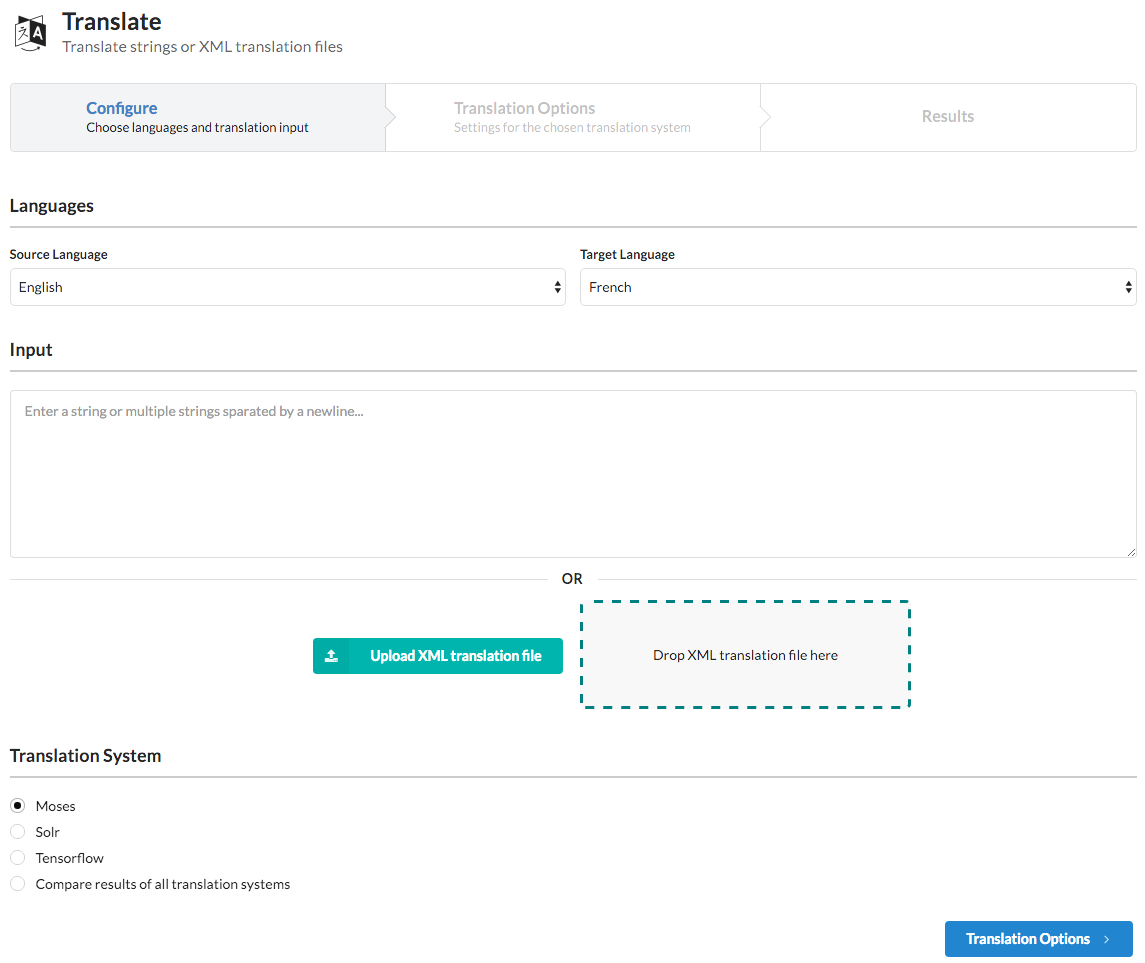
\includegraphics[width=0.9 \textwidth]{images/web_application_index.png}
    \caption{First step: Set source and target languages, translation input and choose the translation system.}
    \label{fig:web_app_index}
\end{figure}


\subsection{Translation Options}

\textbf{Moses}

\begin{itemize}
\item \textbf{Drop unknown words} [No] Words not in the vocabulary are either dropped or replaced by the word in the source language.
\item \textbf{Search algorithm} [Normal Stack] Beside the stack based ``Beam sarch'', Moses implemented ``Cube Pruning''. The latter should perform a bit faster than the default algorithm.
\item \textbf{Verbose} [2] Verbosity level of the debug output.
\item \textbf{Stack size} [100] Number of hypotheses kept on each stack while decoding.
\item \textbf{Tune weights manually} [No] If enabled, the four weights for the translation models can be set manually. Normally, these weights are optimized automatically after tuning.
\end{itemize}
\textbf{Baseline System (Solr)}

\begin{itemize}
\item \textbf{Number of Rows} [100] Number of rows returned by Solr when searching for a translation.
\end{itemize}
\textbf{Tensorflow}

\begin{itemize}
\item \textbf{Number of Layers} [2] Number of layers in the neural networks.
\item \textbf{Size} [256] Number of Cells in each layer.
\end{itemize}
Note that the provided parameters must match a model that was trained with the same values, otherwise Tensorflow will fail to load the model.

\section{Architecture}

Each translation system implements a common interface (see UML in Figure \ref{fig:web_app_uml}). This makes it easy to support additional translation engines at any time.

\begin{figure}[H]
    \centering
    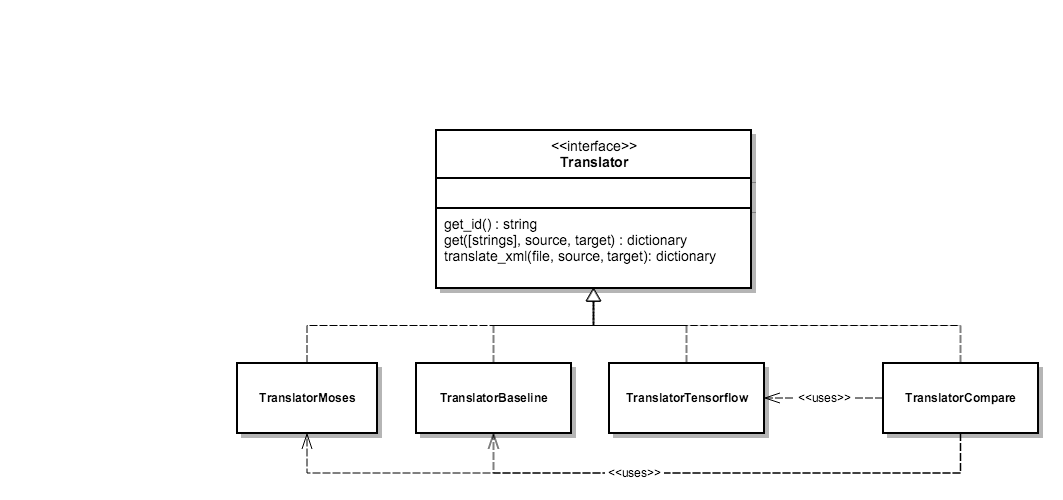
\includegraphics[width=1.0 \textwidth]{images/web_application_uml.png}
    \caption{High level overview of the application. Each translation system implements the ``Translator'' interface. The class ``TranslatorCompare'' is special in a way that it gets the translations from all implemented systems so that the results can be compared next to each other.}
    \label{fig:web_app_uml}
\end{figure}

The backend offers a REST based interface for the different functionalities. The frontend communicates through Ajax requests with that interface and handles the JSON responses accordingly.

\begin{figure}[H]
    \centering
    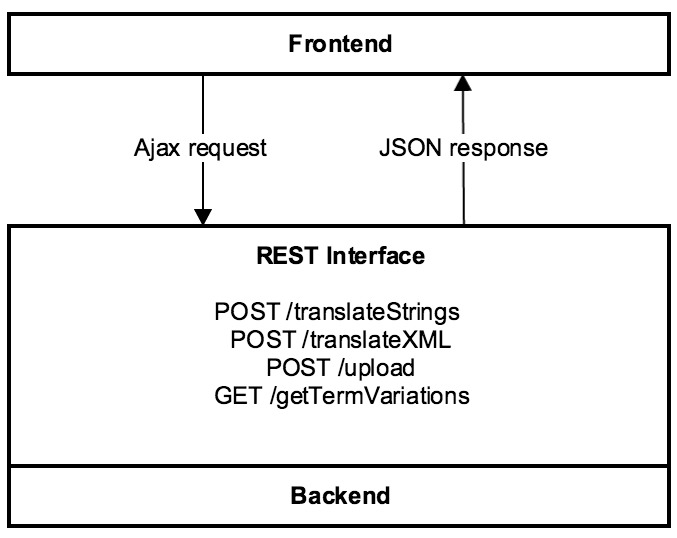
\includegraphics[width=1.0 \textwidth]{images/web_application_rest.png}
    \caption{Graphical visualization how the frontend communicates with the backend through a REST interface.}
    \label{fig:web_app_uml}
\end{figure}

We decided to implement the business logic with Python\footnote{Python programming language: \url{https://www.python.org/}}. The REST interface is powered by a microframework called ``Flask''\footnote{Flask, a Python microframework:  \url{http://flask.pocoo.org/}}. Flask has a built-in server and offers RESTful request dispatching, among many other features. Table xy shows the possible endpoints together with the expected request data and response. Note that the business logic is completely independent from Flask.

\begin{table}[H]
\centering
\begin{tabular}{@{}lll@{}}
\toprule
Endpoint                                                           & Request Data                                                                                                                                                                                                                                                                                  & Response                                                                                                                                                                            \\ \midrule
\begin{tabular}[c]{@{}l@{}}translateStrings \\ (POST)\end{tabular} & \begin{tabular}[c]{@{}l@{}}decoder: The ID of the translation system to use\\ decoder\_settings: Settings for decoding (JSON)\\ strings: Array of strings to translate\\ lang\_from: Source language code (e.g. 'en')\\ lang\_to: Target language code (e.g. 'fr')\end{tabular} & \begin{tabular}[c]{@{}l@{}}translations: List of translations, index matches input strings\\ debug: Debug output from the decoding process\end{tabular}                             \\ \midrule
\begin{tabular}[c]{@{}l@{}}translateXML\\ (POST)\end{tabular}      & \begin{tabular}[c]{@{}l@{}}decoder: The ID of the translation system to use\\ decoder\_settings: Settings for decoding (JSON)\\ xml\_filename: Hashed filename of the \\ previous uploaded XML file\\ lang\_from: Source language code\\ lang\_to: Target language code\end{tabular}             & \begin{tabular}[c]{@{}l@{}}translations: JSON object with translation key, source string and corresponding translation\\ debug: Debug output from the decoding process\end{tabular} \\ \midrule
\begin{tabular}[c]{@{}l@{}}getTermVariations\\ (GET)\end{tabular}  & \begin{tabular}[c]{@{}l@{}}source: Source language code\\ target: Target language code\\ term: String in source language\end{tabular}                                                                                                                                                         & Array for each found variation, together with its count                                                                                                                             \\ \midrule
\begin{tabular}[c]{@{}l@{}}upload\\ (POST)\end{tabular}            & file: Data from uploaded XML translation file                                                                                                                                                                                                                                                 & \begin{tabular}[c]{@{}l@{}}success: True oder False\\ filename: A hashed filename of the uploaded XML file\end{tabular}                                                            
\end{tabular}
\caption{My caption}
\label{my-label}
\end{table}

The frontend uses AngularJS\footnote{\url{https://angularjs.org/}} together with the Semantic UI\footnote{\url{http://semantic-ui.com/}} CSS framework.

% com.ancestry.android.apps.ancestry_your_capitalized
% com.google.android.apps.plus_collexion_abuse_appeal_rejected
% com.google.android.apps.plus_collexion_suspension_details
% --data_binary '{"id":"com.google.android.apps.plus_collexion_abuse_appeal_rejected","value":{"set":"votre"},"value_lc":{"set":"votre"}}'


\chapter{Evaluation}

How can we automatically measure the quality of machine translated text? There exists an algorithm called ``BLEU'' \cite{bleu_score} which is mostly used for this task. We first shortly describe how BLEU works, then explain our evaluation setup and finally present the BLEU scores achieved for the different translation systems.

\section{BLEU (Bilingual Evaluation Understudy)}


``The closer a machine translation is to a professional human translation, the better it is.`` This is the central idea behind the BLEU algorithm \citep{bleu_score}. BLEU computes a score by comparing machine translated sentences (called ``candiates'') against single or multiple reference translations. The score is averaged over the whole corpus to estimate the overall translation quality. The output of BLEU  is a number between 0 and 1 that indicates the similarity of the candidate and reference translations. The closer a value is to 1, the more similar are the texts. %A value of 1 means that the candidate and reference translations are identical. 

\subsection{Algorithm}

BLEU compares \(n\)-grams of the candidate with \(n\)-grams of the reference translation and counts the number of matches. These matches are position-independent. The more the matches, the better the candidate translation is. \citep{bleu_score}.

The score is based on a modified \(n\)-gram precision. One counts up the maximum number of times a \(n\)-gram occurs in any single reference translation. Next, one clips the total count of each candidate \(n\)-gram by its maximum reference count: \( count_{clip} = min(count, max\_ref\_count) \). The clipped counts for all \(n\)-grams are added up and divided by the total number of candidate words \citep{bleu_score}.
\\
\\
\textbf{Example} Consider this example from \cite{bleu_score} that computes a modified unigram precision:

\begin{itemize}
\item Candidate: \underline{the} \underline{the} the the the the the
\item Reference 1: \underline{The} cat is on \underline{the} mat.
\item Reference 2: There is a cat on the mat.
\end{itemize}
The word ``the'' appears twice in the first reference and once in the second reference, it is therefore clipped to:
\( count_{clip} = min(7, 2) = 2 \). The final modified unigram precision is \( P = \frac{2}{7} \).

To compute the modified precision score \(p_n\) for the entire corpus, we compute the \(n\)-gram matches for each sentence. Next, the clipped \(n\)-gram counts for all candidates are added up and divided by the number of candidate \(n\)-grams in the corpus:

\[  p_n = \frac{\sum_{C\in\{Candidates\}} \sum_{n-gram \in C} count_{clip}(n-gram)}{\sum_{C'\in\{Candidates\}} \sum_{n-gram' \in C'} count(n-gram')}   \]
In order to prevent very short candidates from receiving a too high  precision score, a ``brevity penalty'' is introduced. The penalty is 1.0 if the candidate's length is the same as any reference translation's length. We call the closest reference sentence length the ``best match length''. The brevity penalty is computed over the entire corpus. First, we compute the reference lengths \(r\) by summing the best match lengths for each candidate sentence in the corpus. We choose the brevity penalty to be a decaying exponential in \(r/c\), where \(c\) is the total length of the candidate translation corpus \cite{bleu_score}.

The final BLEU score is a combination of the brevity penalty \(PB\) and the geometric mean of the modified precision scores \(pn\) of the corpus:

\[  BP = \begin{cases}1 & c > r\\e^{(1-\frac{r}{c})} & c \leq r\end{cases} \]

\[ BLEU = BP \: exp \left(  \sum_{n=1}^N w_n \:  log \: p_n \right) \]
The baseline in \citep{bleu_score} used \(N = 4 \) and uniform weights  \( w_n = 1/N \). 

\section{Setup}

The BLEU scores were computed in different evaluation runs for the results of translating English to French and German. We used k-fold cross-validation to predict how the different models would perform if they were applied to independent data. The parallel corpus was split into 6 equal sized samples. One sample was always reserved as development set for Moses (Tuning) and Tensorflow, the remaining 5 samples were used to evaluate BLEU. For each evaluation run, four samples were merged into training data and a single sample was used as test set (see Figure \ref{fig:evaluation_k_fold}).

\begin{figure}[H]
    \centering
    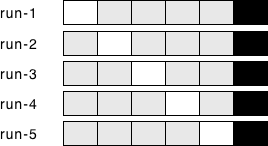
\includegraphics[width=0.3 \textwidth]{images/evaluation_k_fold_cross_validation.png}
    \caption{Graphic showing how the parallel corpus was split  for the different evaluation runs. The white rectangle represents the test data, grey means training data and the black rectangle is the fixed development sample.}
    \label{fig:evaluation_k_fold}
\end{figure}

The Baseline System needed a special setup. First of all, the development set is ignored since there is no evaluation or tuning involved in this model. Secondly, we needed to index the training data for each evaluation run separately into Solr. This was achieved by creating new cores in Solr according to the following schema:

\[ source-target-run-k-(source|target) \]
where \(source\) and \(target\) are the source and target language and \(k\) is the index of the evaluation run (1-5). For example, in the first evaluation run for translating English to French, the French training data is put into the core ``en-fr-run-1-fr''.

\section{BLEU Scores}

The left table shows BLEU scores achieved for translating English to French, the right one for English to German. We used a perl script\footnote{Script to calculate BLEU score: \url{multi-bleu.perl}} included in Moses to compute the scores. As proposed in \citep{bleu_score}, \(n\)-grams up to \(n=4\) are considered in the calculation. Our corpus offers only one reference translation since apps are not translated multiple times into the same language. Note that the BLEU scores are reported as percentages. This format is the output of the script and seems mostly used in machine translation literature.

\subsection{Moses}

\begin{table}[H]
\centering
\begin{minipage}{0.48\textwidth}
\centering
\begin{tabular}{@{}lr@{}}
\toprule
EN-FR & BLEU          \\ \midrule
run-1 & 47.45          \\
run-2 & 53.19          \\
run-3 & 49.91          \\
run-4 & 51.5           \\
run-5 & 51.74          \\
\textbf{\o}      & \textbf{50.76} \\
 \(\sigma\)     & 1.95           \\ \bottomrule
\end{tabular}
\label{my-label}
\end{minipage}
\hfill
\begin{minipage}{0.48\textwidth}
\centering
\begin{tabular}{@{}lr@{}}
\toprule
EN-DE & BLEU          \\ \midrule
run-1 & 41.6          \\
run-2 & 44.53          \\
run-3 & 44.12          \\
run-4 & 46           \\
run-5 & 43.73          \\
\textbf{\o}      & \textbf{44.00} \\
 \(\sigma\)     & 1.42           \\ \bottomrule
\end{tabular}
\label{my-label}
\end{minipage}
\end{table}

\subsection{Tensorflow}

\begin{table}[H]
\centering
\begin{minipage}{0.48\textwidth}
\centering
\begin{tabular}{@{}lrrrr@{}}
\toprule
EN-FR & BLEU\footnote{2 Layers, 256 Units, 40'000 words} &  BLEU\footnote{3 Layers, 512 Units, 40'000 words}     & BLEU\footnote{1 Layers, 128 Units, 40'000 words} & BLEU\footnote{2 Layers, 256 Units, 50'000 words} \\ \midrule
run-1 			& 19.86  			&   19.36			&	 23.13 			& 20.53     			\\
run-2 			& 26.7   			&   21.29    		&	25.68			& 22.44	\\
run-3 			& 25.27  			&   19.57    		&	23.2				& 21.07	\\
run-4 			& 20.64  			&   20.58    		&	20.48			& 26.86	\\
run-5 			& 27.43  			&   21.42  			&	22.21			& 28.49	\\
\textbf{\o}    	& \textbf{23.98} 	&  	\textbf{20.44}	&	\textbf{22.94}	& \textbf{23.88}	\\
 \(\sigma\)    	& 3.13           	&	0.85				&	1.68				& 3.2	\\ \bottomrule
\end{tabular}
\label{my-label}
\end{minipage}
\hfill
\begin{minipage}{0.48\textwidth}
\centering
\begin{tabular}{@{}lrrrr@{}}
\toprule
EN-DE & BLEU\footnote{2 Layers, 256 Units, 40'000 words} &  BLEU\footnote{3 Layers, 512 Units, 40'000 words}     & BLEU\footnote{1 Layers, 128 Units, 40'000 words} & BLEU\footnote{2 Layers, 256 Units, 50'000 words} \\ \midrule
run-1 			& 18.72  			&   18.58			&	20.02 			& 25.56     			\\
run-2 			& 23.95   			&   20.34    		&	19.93			& 24.13	\\
run-3 			& 22.14  			&   19.96    		&	22.04			& 23.62	\\
run-4 			& 19.66  			&   18.82    		&	19.86			& 26.87	\\
run-5 			& 17.03  			&   19.71  			&	20				& 24.11	\\
\textbf{\o}    	& \textbf{20.3} 	&  	\textbf{19.48}	&	\textbf{20.37}	& 	\textbf{24.86}	\\
 \(\sigma\)    	& 2.46           	&	0.67				&	0.84				& 1.2	\\ \bottomrule
\end{tabular}
\label{my-label}
\end{minipage}
\end{table}

\subsection{Baseline System}

\begin{table}[H]
\centering
\begin{minipage}{0.48\textwidth}
\centering
\begin{tabular}{@{}lr@{}}
\toprule
EN-FR & BLEU          \\ \midrule
run-1 & 25.08          \\
run-2 & 29.28          \\
run-3 & 25.35          \\
run-4 & 26.2           \\
run-5 & 25.7          \\
\textbf{\o}      & \textbf{26.32} \\
 \(\sigma\)     & 1.53           \\ \bottomrule
\end{tabular}
\label{my-label}
\end{minipage}
\hfill
\begin{minipage}{0.48\textwidth}
\centering
\begin{tabular}{@{}lr@{}}
\toprule
EN-DE & BLEU          \\ \midrule
run-1 & 8.74          \\
run-2 & 9.57          \\
run-3 & 9.03          \\
run-4 & 9.68           \\
run-5 & 8.98          \\
\textbf{\o}      & \textbf{9.2} \\
 \(\sigma\)     & 0.36           \\ \bottomrule
\end{tabular}
\label{my-label}
\end{minipage}
\end{table}


\section{Observations}

\chapter{Conclusion and Future Work}


%\chapter{The Problem}
%In which we understand what the problem is in detail.
%
%\chapter {The Solution}
%In which you describe your solution.
%
%\chapter {The Validation}
%In which you show how well the solution works.
%
%\chapter {Conclusion and Future Work}
%In which we step back, have a critical look at the entire work, then conclude, and learn what lies beyond this thesis.





%END Doc
%-------------------------------------------------------

\bibliography{thesis}
\bibliographystyle{plain}


\end{document}
